\documentclass[class=jsarticle, crop=false, dvipdfmx, fleqn]{standalone}
%% preamble for Numerical-structure-analysis report

\input{/Users/User/Documents/Project/TeX/preamble/mypreamble}

%% titles
\title{先端データ解析論 レポート}
\author{37-196360 \quad 森田涼介}


%% setting for listings
\newtcbinputlisting[auto counter]{\reportlisting}[3][]{%
	listing file = {#3},
	listing options = {language=python, style=tcblatex, numbers=left, numberstyle=\tiny},
	listing only,
	breakable,
	toprule at break = 0mm,
	bottomrule at break = 0mm,
	left = 6mm,
	sharp corners,
	drop shadow,
	title = Listings \thetcbcounter : \texttt{#2},
	label = #1,
	}



%% title format
\usepackage{titlesec}
\titleformat{\section}{\LARGE}{宿題\thesection}{0zw}{}
\newcommand{\sectionbreak}{\clearpage}
\titleformat{\subsection}{\Large}{\Alph{subsection})}{0zw}{}

\begin{document}
\section{}

適当な類似度行列に対して局所性保存射影を実装する。

目的関数は,
\begin{equation}
    J = \frac{1}{2} \sum_{i, i' = 1}^{n} W_{i, i'} ||\bm{T} \bm{x}_i - \bm{T} \bm{x}_{i'}||^2
        = \mathrm{tr}\qty(\bm{TXLX}^\mathrm{T} \bm{T}^\mathrm{T})
\end{equation}
であり,
拘束条件は
\begin{equation}
    \bm{TXDX}^\mathrm{T} \bm{T}^\mathrm{T} = \bm{I}
\end{equation}
である。
\(J\)を最小にするような\(\bm{T}\)を求めることを考える。
これはまず,次の一般化固有値問題を解けばよい。
\begin{align}
    & \bm{XLX}^\mathrm{T} \bm{\xi} = \lambda \bm{XDX}^\mathrm{T} \bm{\xi} \\
    & \lambda_1 \ge \cdots \ge \lambda_d \\
    & \bm{\xi}_j^\mathrm{T} \bm{XDX}^\mathrm{T} \bm{\xi}_j = 1
\end{align}
ここから,下位\(m\)個の一般化固有ベクトルを並べ,
\begin{equation}
    \bm{T} = \bm{T}_\mathrm{LPP} = \qty(\bm{\xi}_d,\ \cdots,\ \bm{\xi}_{d-m+1})^\mathrm{T}
\end{equation}
とすればよい。

また,類似度行列にはガウスカーネル
\begin{align}
    & K(\bm{x},\ \bm{c}) = \exp(- \frac{||\bm{x} - \bm{c}||^2}{2 h^2}) \\
    & \bm{W} = \bm{K} =
        \begin{bmatrix}
            K(\bm{x}_1,\ \bm{x}_1) & \cdots & K(\bm{x}_{n},\ \bm{x}_1) \\
            \vdots & \ddots & \vdots \\
            K(\bm{x}_{n},\ \bm{x}_1) & \cdots & K(\bm{x}_{n},\ \bm{x}_{n})
        \end{bmatrix}
\end{align}
を用いることとする。

\(h = 1.0\)としてこれを実装したものが,
\pageref{listing:assignment2}ページのListing \ref{listing:assignment2}である。
結果は図\ref{fig:result1},\ref{fig:result2}に示した通りである。
これより,元のデータのクラスタ構造がうまく保存されたまま次元が削減されていることがわかる。

\begin{figure}[H]
    \centering
    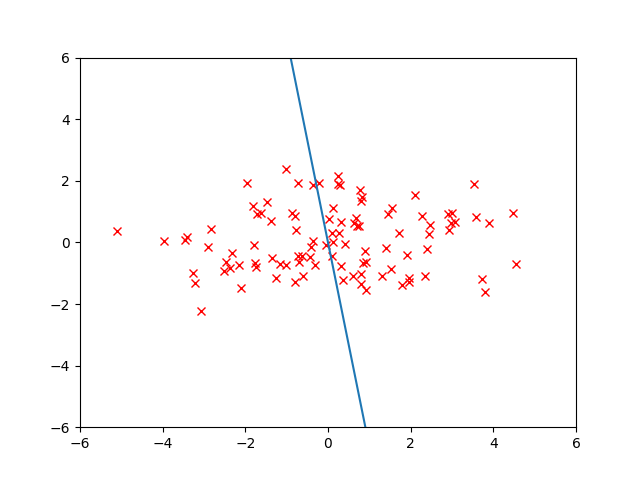
\includegraphics[clip, width=12cm]{../figures/assignment2_result_data1}
    \caption{データ1に対する結果}
    \label{fig:result1}
\end{figure}

\begin{figure}[H]
    \centering
    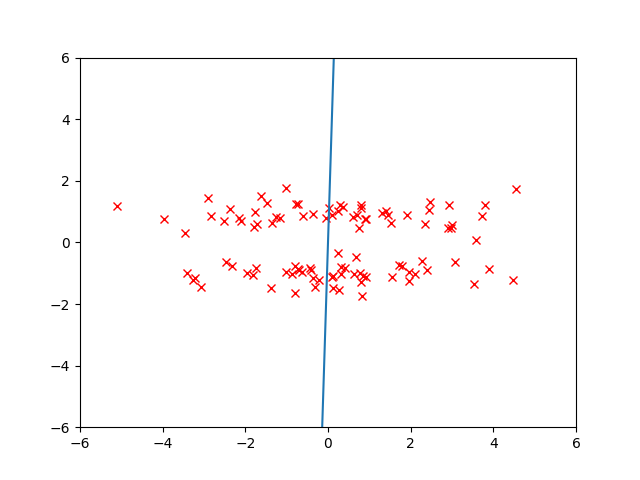
\includegraphics[clip, width=12cm]{../figures/assignment2_result_data2}
    \caption{データ2に対する結果}
    \label{fig:result2}
\end{figure}


\end{document}
